\section{Preprocesado de imágenes}
Inicialmente se diseñó un código para extraer fotografías desde un directorio, etiquetas desde un documento con extensión \textit{.xlsx} y luego transformarlos en matrices de datos que para poder ser utilizados en los proceso de \textit{Machine Learning}. Para la realización de este código, se utilizaron las siguientes librerías: \textit{OS}, \textit{CV2 (OpenCV)}, \textit{Numpy} y \textit{Pandas}. Además de esto el proceso para la realización del código fue el siguiente: 

\subsection{Transformación de fotografías}
En este caso, se utilizó la librería \textit{OS} para crear una lista con nombres en formato cadena de los archivos en un directorio dado. Luego, utilizando la librería \textit{Numpy}, se creó una matriz de ceros para guardar todas las fotografías convertidas en formato de matriz. Para realizar la conversión, previamente se realizó una prueba para obtener las dimensiones mínimas con las que puede trabajar la cámara integrada con la librería \textit{CV2}, cuyo tamaño es 320 $\times$ 180 píxeles. Después, dentro de un bucle \textit{for} se utilizó la librería \textit{CV2} obtener la matriz de pixeles de cada fotografía, ajustar el tamaño a las dimensiones encontradas y luego transformar el canal de color por defecto BGR \textit{(Blue, Green, Red)} a RGB \textit{(Red, Green, Blue)}. 

\subsection{Transformación de etiquetas}

Para transformar las etiquetas en matrices de datos, únicamente se requirió la librería \textit{Pandas}, ya que nos permite utilizar una función específica para leer documentos con formato \textit{.xlsx}, así como acceder a las hojas y columnas del documento. Al guardar el resultado de esta función el siguiente paso es convertirlo a un formato de matriz con funciones de \textit{Numpy}. 

\subsection{Exportación de datos finales}

Antes de realizar la exportación de datos, es importante aplicar una transformación de tipo flotante a entero, en las matrices, y de esta manera se ahorra espacio en el disco duro. Ahora bien, la librería \textit{Numpy} cuenta con una función para exportar matrices de datos de manera individual (una variable a la vez), o bien agruparlas en un solo archivo. En este caso, dado que se necesitan realizar diferentes pruebas, se estará exportando de manera individual, en cambio para los resultados finales, se utilizará la función de guardar de manera agrupada. 

\subsection{Filtrado de imágenes (Modelo No. 8)}
Luego de las pruebas con los primeros 7 modelos de reconocimiento facial, dónde únicamente se utilizaban los datos de las fotografías a un tamaño de 320 $\times$ 180 píxeles, con canal RGB, para alimentar el proceso, se decidió utilizar la librería \textit{OpenCV} para aplicar filtros de bordes a las fotografías, de tal manera que el modelo de aprendizaje no tome en cuenta los colores sino únicamente los bordes de los rostros. Este proceso se aplicó en la sección del código par transformar las fotografías, y en la sección que recopila la imagen en tiempo real. 

\section{Entrenamiento de modelos de \textit{machine learning}}
Para las primeras pruebas se utilizó el framework \textit{TensorFlow y Keras} para poder realizar los diferentes modelos de \textit{Machine Learning} para reconocimiento de orientación de cabeza, utilizando las matrices de datos obtenidas a partir de las bases de datos recopiladas. Para este código se utilizaron las librerías \textit{TensorFlow}, \textit{Matplotlib}, \textit{Numpy} y \textit{Seaborn}. El código fue realizado de la siguiente manera:

\subsection{Extracción de datos previamente procesados}
Luego de exportar los archivos transformados de la base de datos, se generan archivos con extensión \textit{.npy} para los archivos de una variable y \textit{.npz} para los de múltliple variables. Dichos archivos pueden ser importados utilizando también funciones de la librería \textit{Numpy}, para guardarlos en variables utilizables dentro del código, optimizando así el tiempo de transformación de datos.

\subsection{Modelo de reconocimiento de orientación de cabeza}
El primer pasó fue normalizar los valores de las matrices, dado que son imágenes RGB, cada píxel de estas está representado por 3 valores que varían entre 0 y 255, y se necesitan valores entre 0 y 1, por lo que únicamente se tuvo que dividir tanto la variable con datos de entrenamiento y prueba entre el valor 255. 

\subsubsection{Primer grupo de modelos de aprendizaje}
Inicialmente, dado que se trata de un modelo que trabaja con matrices derivadas de fotografías, se utilizó una CNN (Red Convolucional Neurnal), la cual permite detectar patrones en las imágenes. Utilizando \textit{Tensorflow} y \textit{Keras}, se definieron 7 capas para la generación del modelo. En este caso se utilizó en primera instancia una capa convolucional en 2D, con 10 kernels de tamaño 3 $\times$ 3, función de activación \textit{ReLU}, y por ser la primera capa se agregan las dimensiones de entrada (fotografía). Luego, se aplicó una capa con la técnica de \textit{Max Pooling} con tamaño 2 $\times$ 2. Después, se aplica una capa de aplanado previa necesaria para poder utilizar las siguientes capas densas. Esta vez se utilizaron 3 capas densas, con 75, 150 y 75 nodos respectivamente con función de activación \textit{ReLU}. Por último, se aplica una capa densa con una cantidad de nodos definida por el número de clases a utilizar y función de activación \textit{Softmax}. Con esta especificación de hiperparámetros, se procede a unir las capas en un modelo secuencial, para luego compilarlo con un optimizador \textit{Adam}, para la pérdida se utilizó \textit{Sparse categorical crossentropy}, dado que las etiquetas fueron definidas como enteros y no en el formato \textit{One-Hot}. Para finalizar con los hiperparámetros, en la opción métricas se escoge la opción \textit{Accuracy} o precisión. Luego de entrenado el modelo, se procede a guardarlo con la función de guardar en \textit{Keras}, en el cual el argumento es el directorio donde se desea guardar el archivo con extensión \textit{.keras} y poder utilizarlo en otros códigos.

Al tener configurado el modelo, se procede al entrenarlo, guardarlo y exportar las gráficas descriptivas respectivas. En esta etapa se cuenta con 4 modelos que varían dado que se utilizó cada uno de los diferentes grupos de etiquetas. A continuación se muestran las gráficas de pérdida y exactitud para cada modelo, utilizando el grupo de entrenamiento actualizado con las fotografías de Gerardo Fuentes (autor), así como las matrices de confusión utilizando la librería \textit{Seaborn}:

\begin{figure}[H]
	\centering
	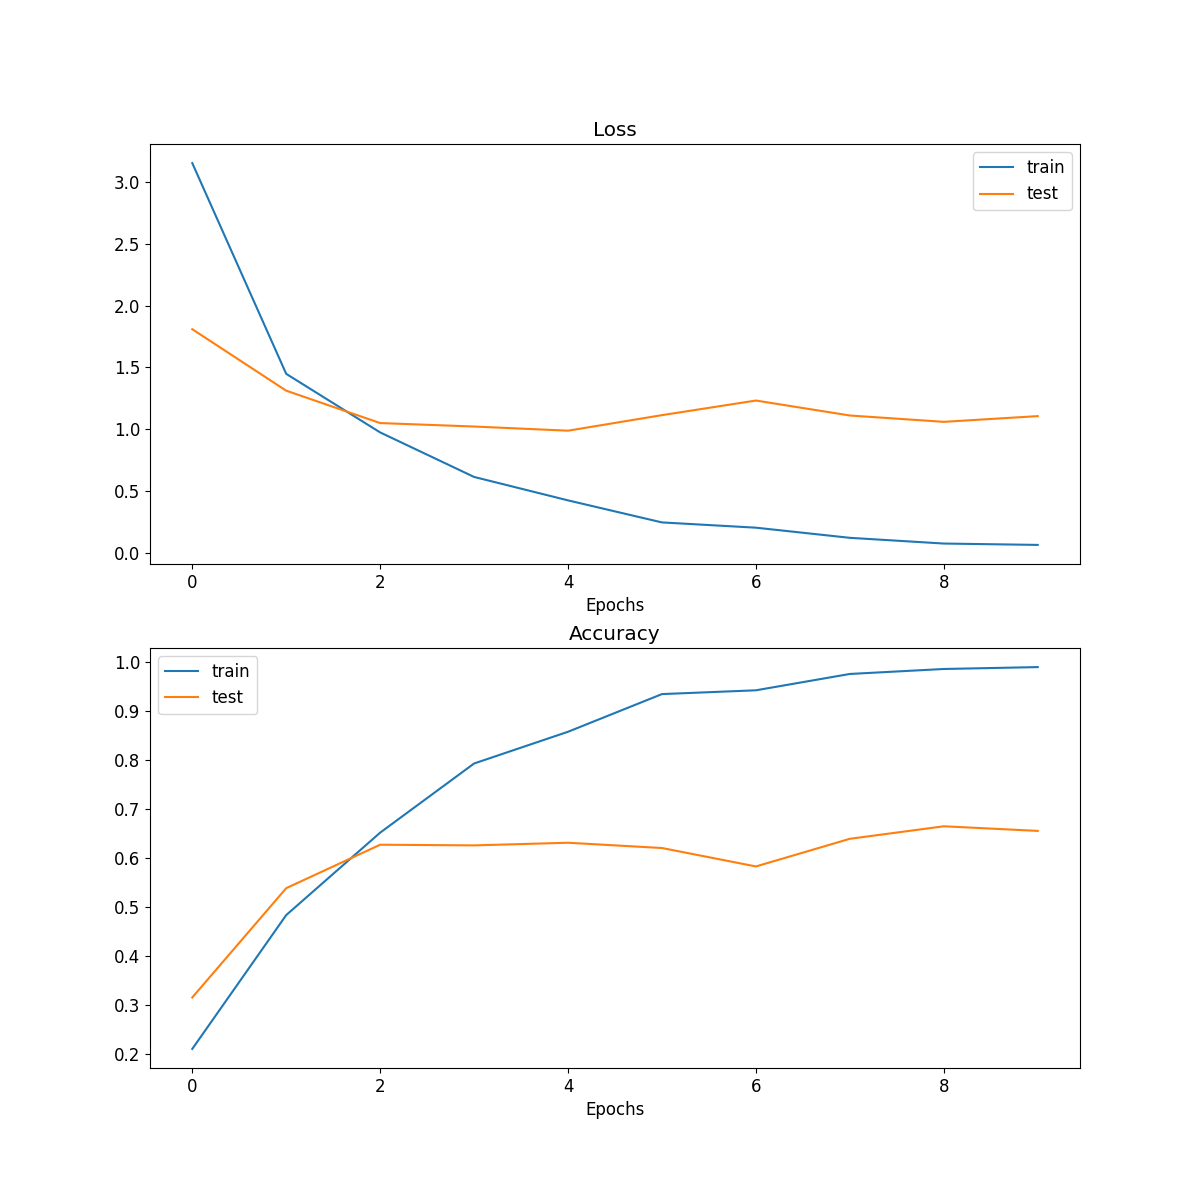
\includegraphics[scale=0.65]{figures/LA0.png}
	\caption{Pérdida y exactitud del primer modelo con 9 clases}
	\label{fig:img9}
\end{figure}

\begin{figure}[H]
	\centering
	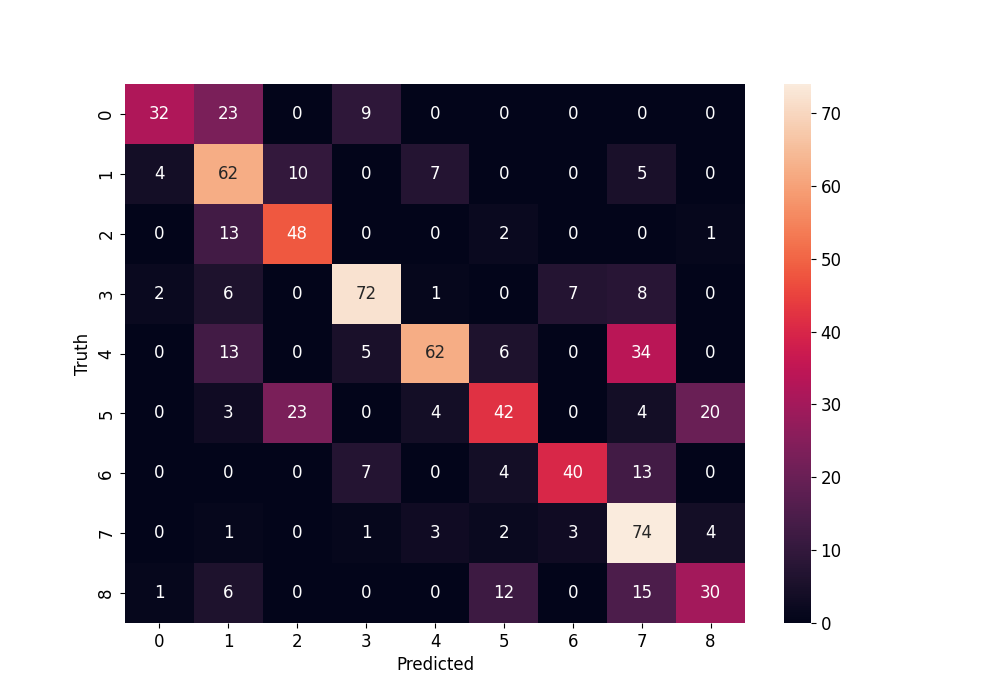
\includegraphics[scale=0.75]{figures/CM0.png}
	\caption{Matriz de confusión del primer modelo con 9 clases}
	\label{fig:img10}
\end{figure}

\begin{figure}[H]
	\centering
	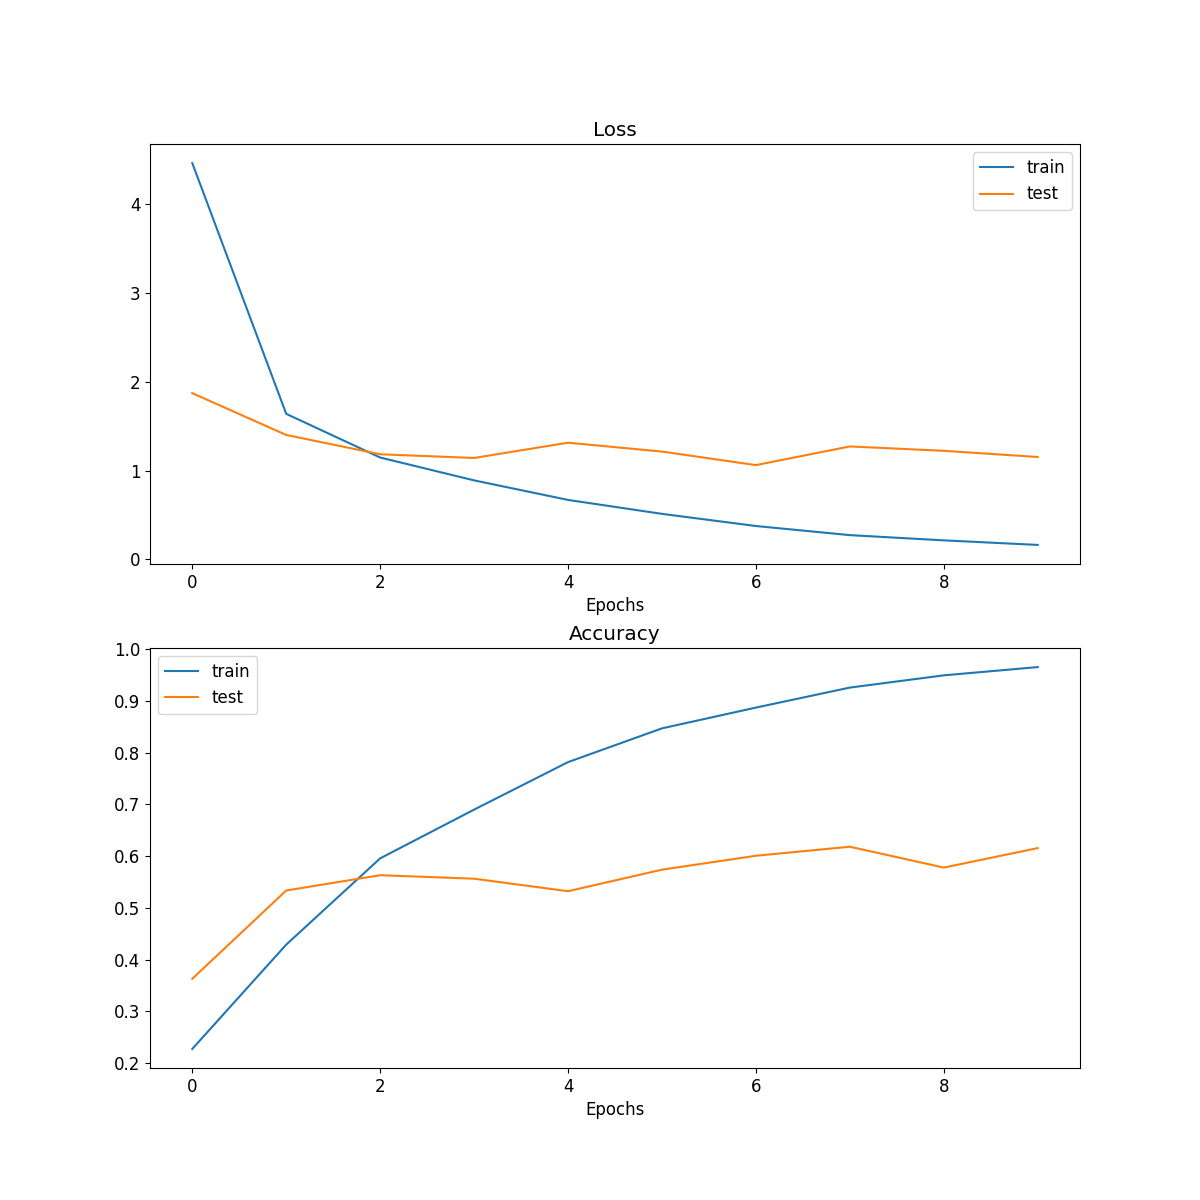
\includegraphics[scale=0.65]{figures/LA1.png}
	\caption{Pérdida y exactitud del segundo modelo con 9 clases}
	\label{fig:img11}
\end{figure}

\begin{figure}[H]
	\centering
	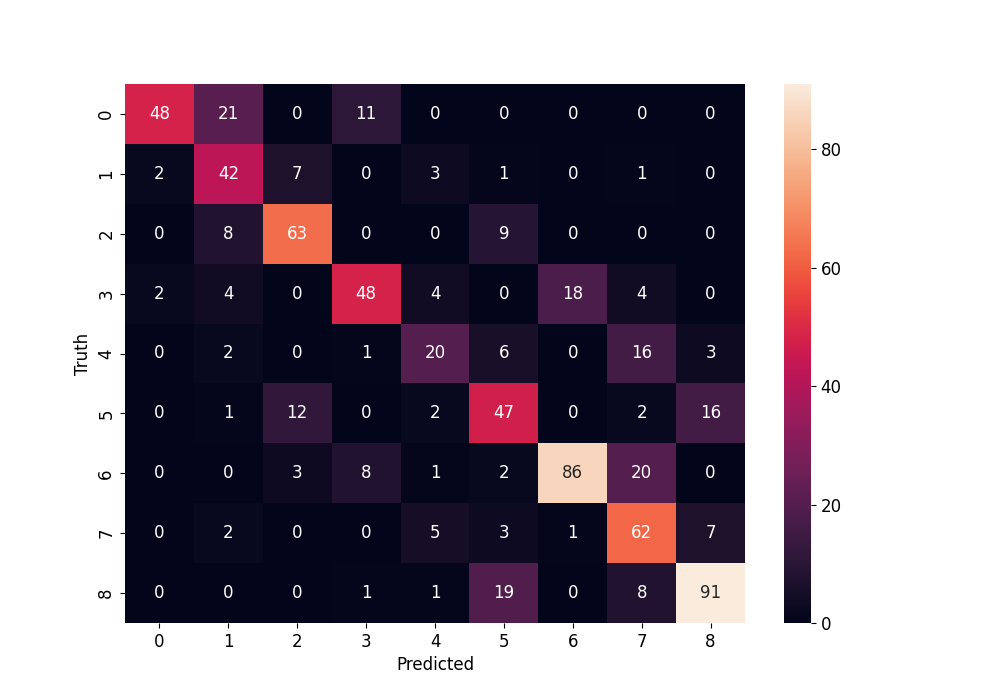
\includegraphics[scale=0.75]{figures/CM1.png}
	\caption{Matriz de confusión del segundo modelo con 9 clases}
	\label{fig:img12}
\end{figure}

\begin{figure}[H]
	\centering
	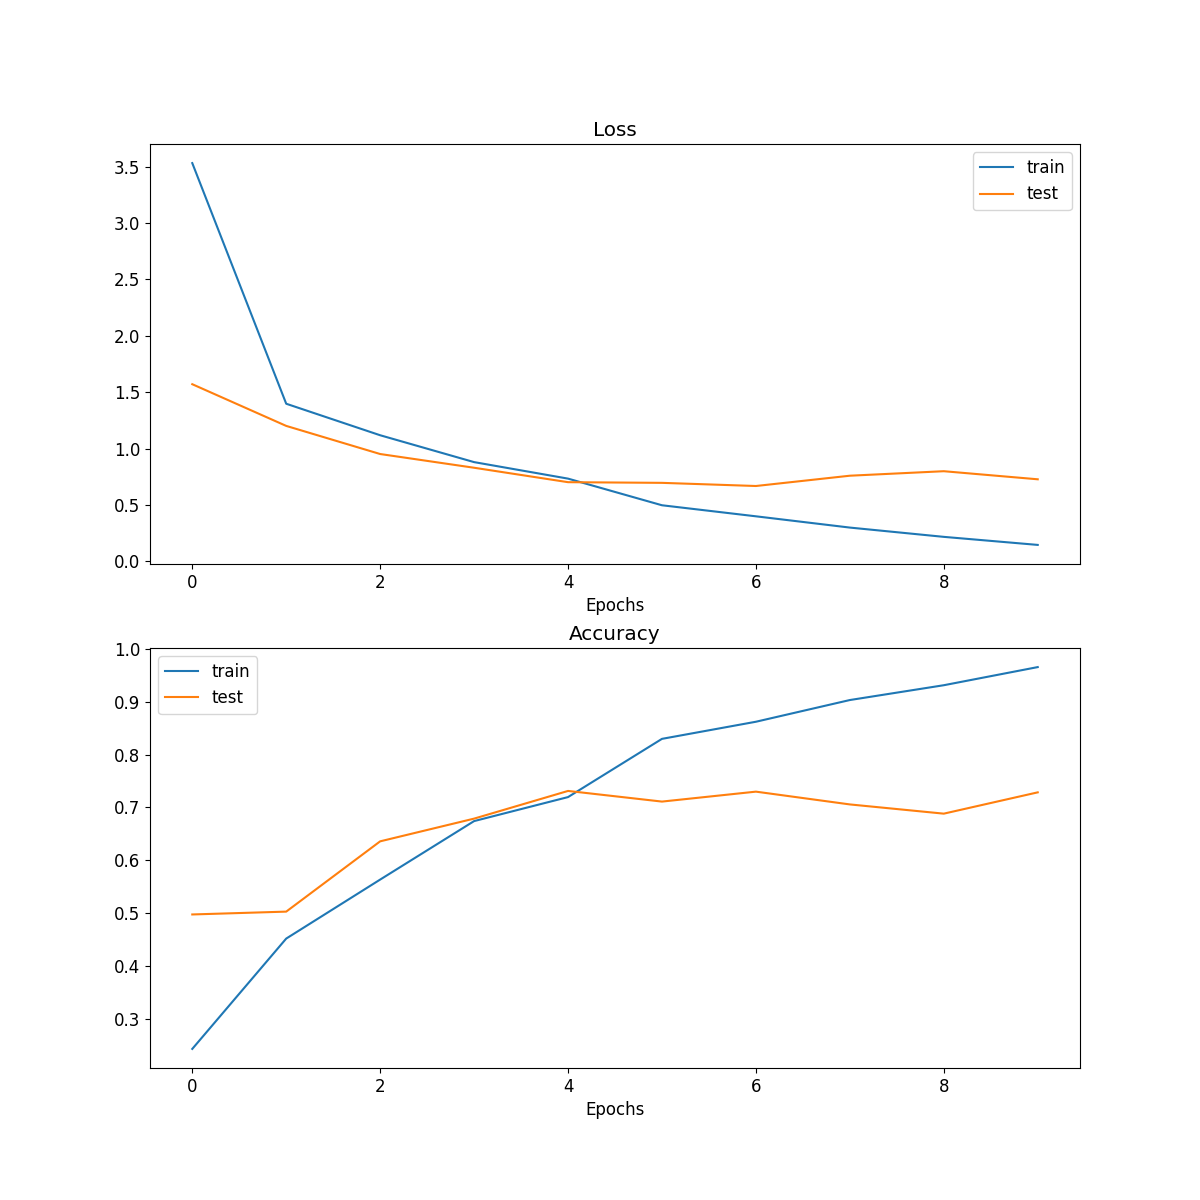
\includegraphics[scale=0.65]{figures/LA2.png}
	\caption{Pérdida y exactitud del primer modelo con 6 clases}
	\label{fig:img13}
\end{figure}

\begin{figure}[H]
	\centering
	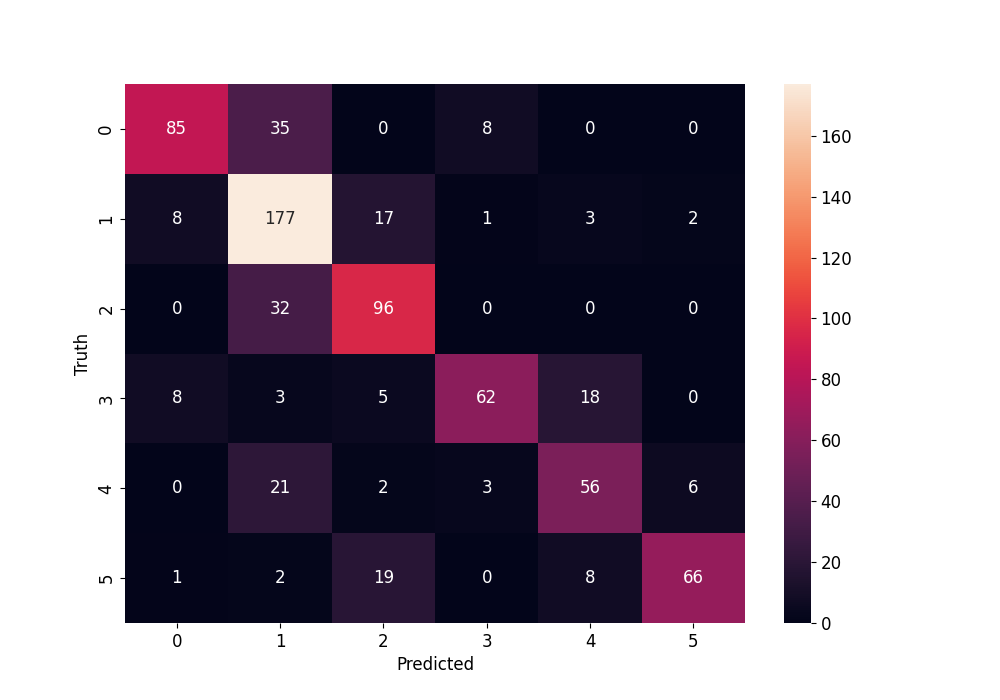
\includegraphics[scale=0.75]{figures/CM2.png}
	\caption{Matriz de confusión del primer modelo con 6 clases}
	\label{fig:img14}
\end{figure}

\begin{figure}[H]
	\centering
	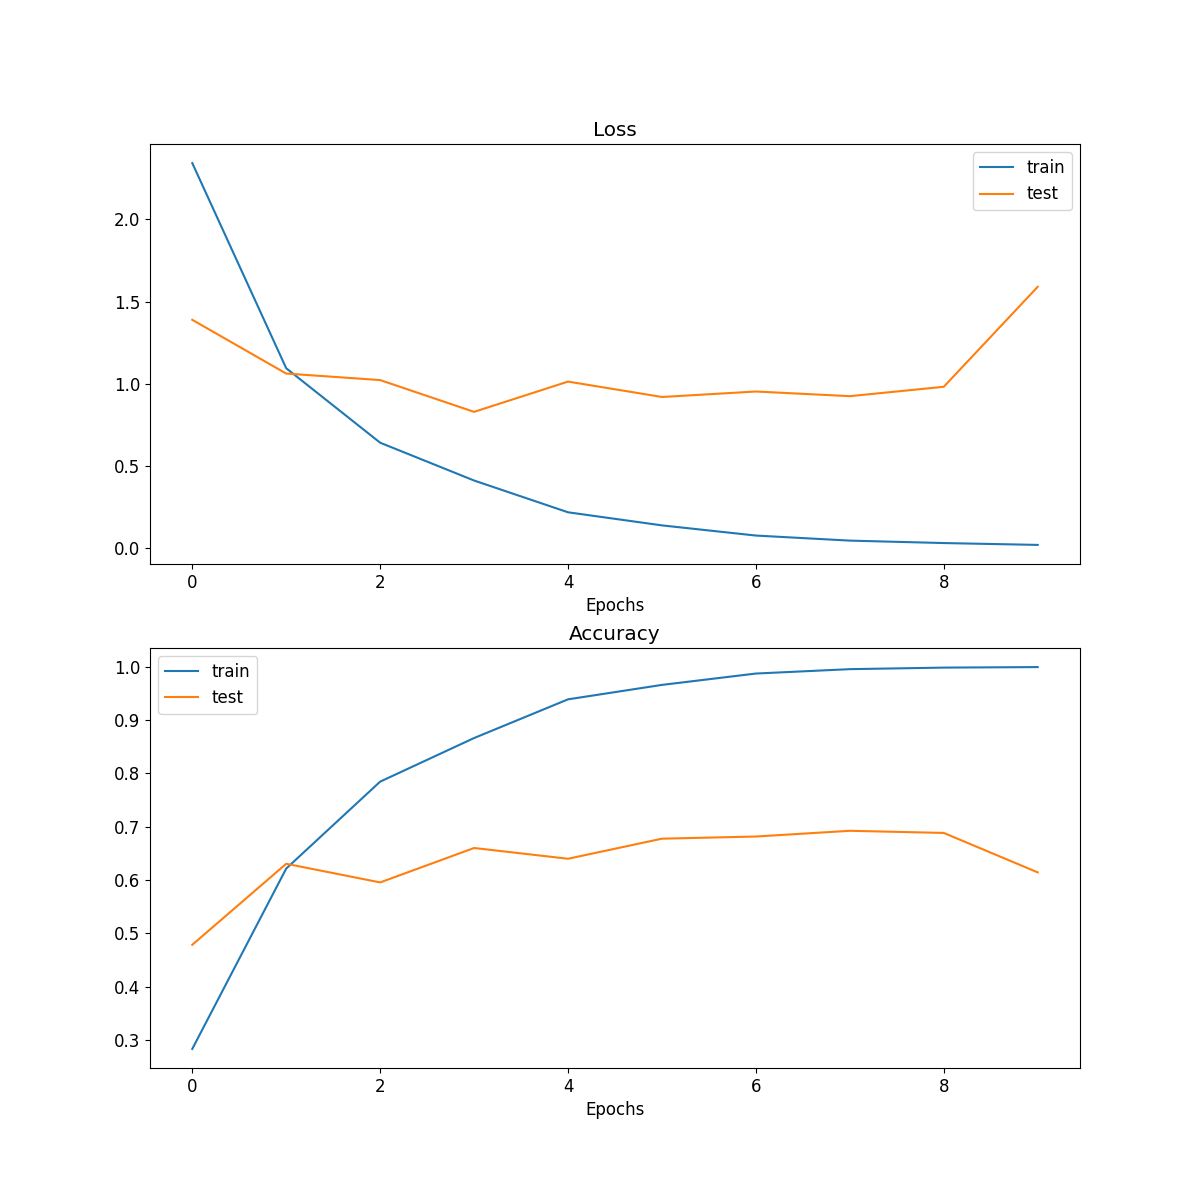
\includegraphics[scale=0.65]{figures/LA3.png}
	\caption{Pérdida y exactitud del segundo modelo con 6 clases}
	\label{fig:img15}
\end{figure}

\begin{figure}[H]
	\centering
	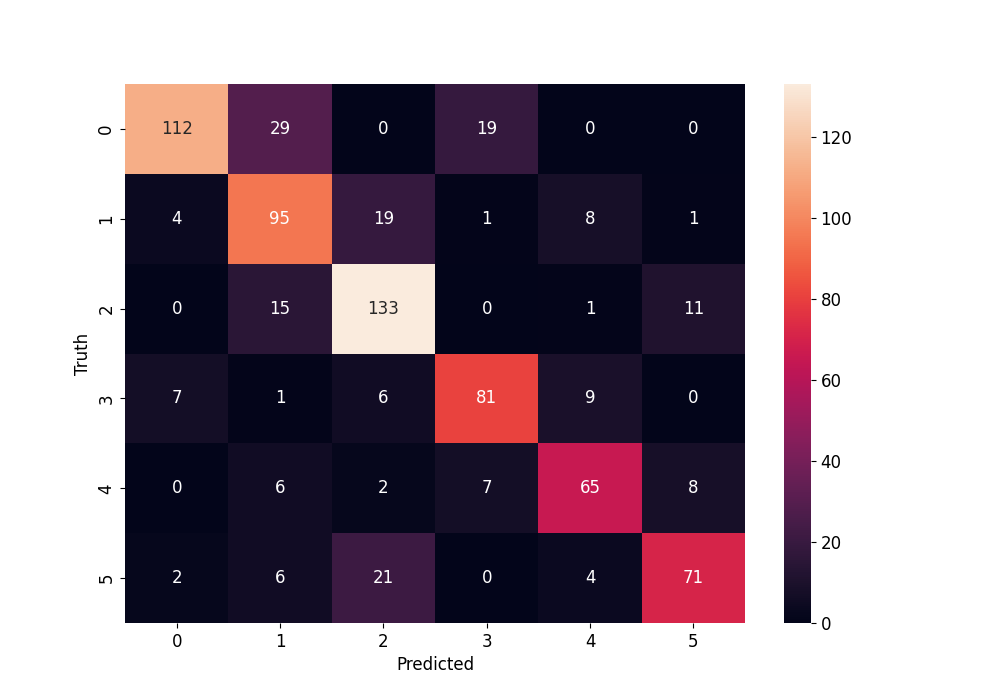
\includegraphics[scale=0.75]{figures/CM3.png}
	\caption{Matriz de confusión del segundo modelo con 6 clases}
	\label{fig:img16}
\end{figure}

En las figuras 9 a las 16 se puede observar que se produce un sobreajuste, tanto en pérdida como en exactitud en todos los modelos entrenados. Los valores en pérdida de validación no disminuyen más allá del valor 1.0 y la exactitud en validación no supera el 70\%. Además, en las matrices de confusión, de todos los modelos, se observa que la predicción falla al detectar la posición vertical. Esto sucede dado que las fotografías de la base de datos ICPR, tienen el mismo fondo en todos su casos. Además, la mayoría de los sujetos de prueba son de sexo masculino, caucásicos y con un rango de edad similar. Además de ser únicamente 11 personas diferentes. Con dichos resultados, se pueden tomar diferentes decisiones. Las acciones a considerar son: 

\begin{itemize}
	\item Conseguir más fotografías y con más diversidad de sujetos y fondos.
	\item Reducir nuevamente la cantidad de clases a 3 o 4. 
	\item Realizar un sobreajuste enfocado en el rostro del usuario.
\end{itemize}

\subsubsection{Segundo grupo de modelos de aprendizaje}
En este caso se utilizó la misma configuración para el modelo de aprendizaje utilizado en los primeros 4 modelos, por lo que únicamente se varió la cantidad de etiquetas utilizadas. A continuación se muestran las gráficas descriptivas para el modelo de 4 clases:

\begin{figure}[H]
	\centering
	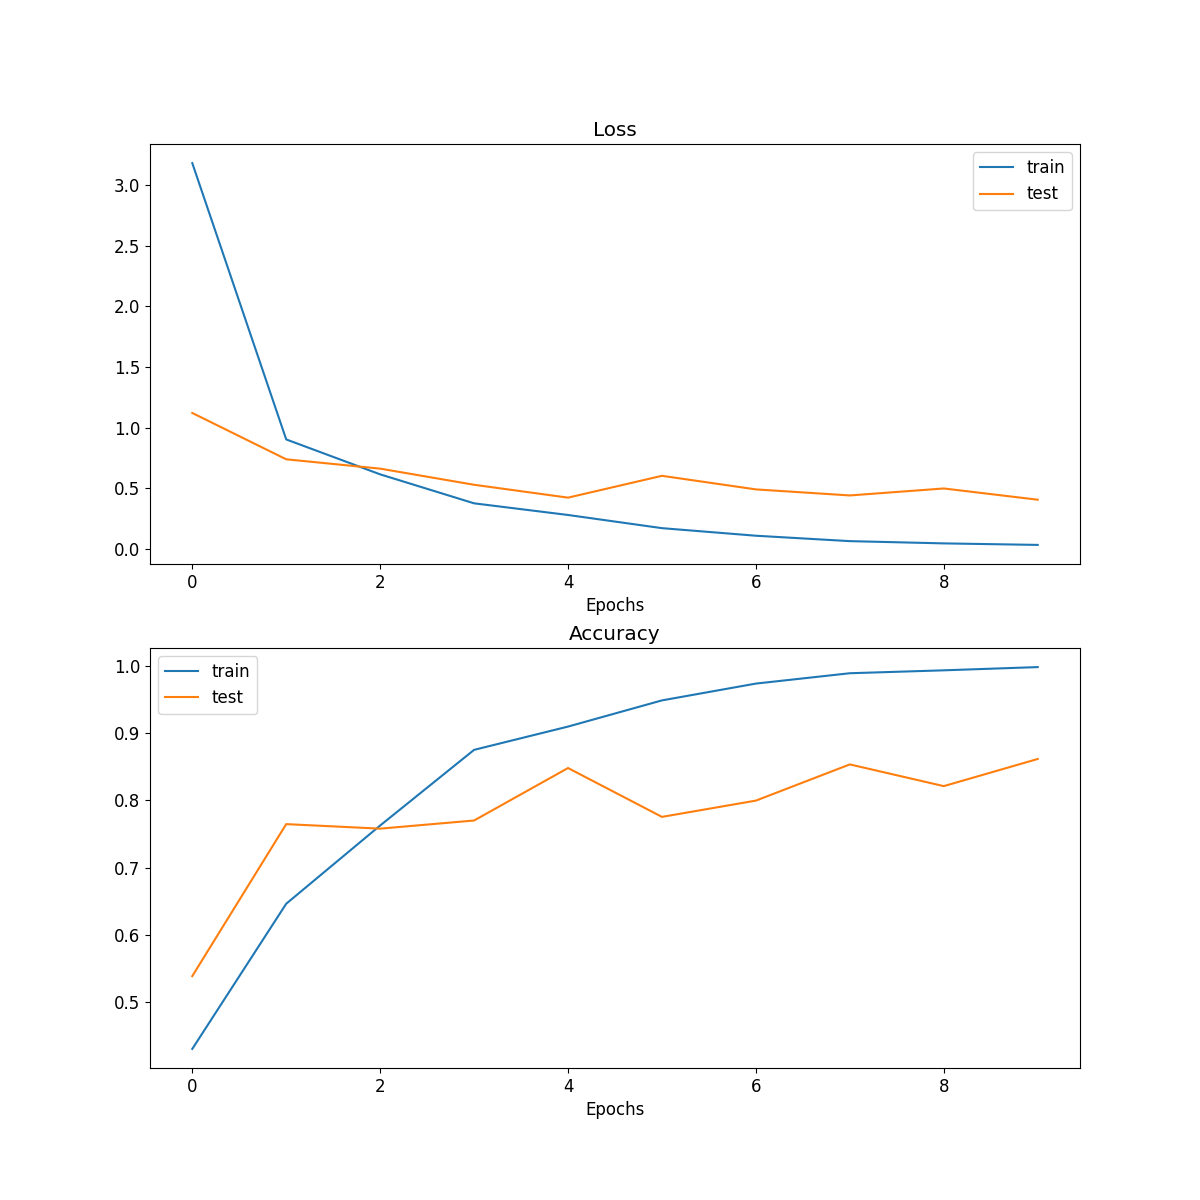
\includegraphics[scale=0.65]{figures/LA4.png}
	\caption{Pérdida y exactitud del modelo con 4 clases}
	\label{fig:img17}
\end{figure}

\begin{figure}[H]
	\centering
	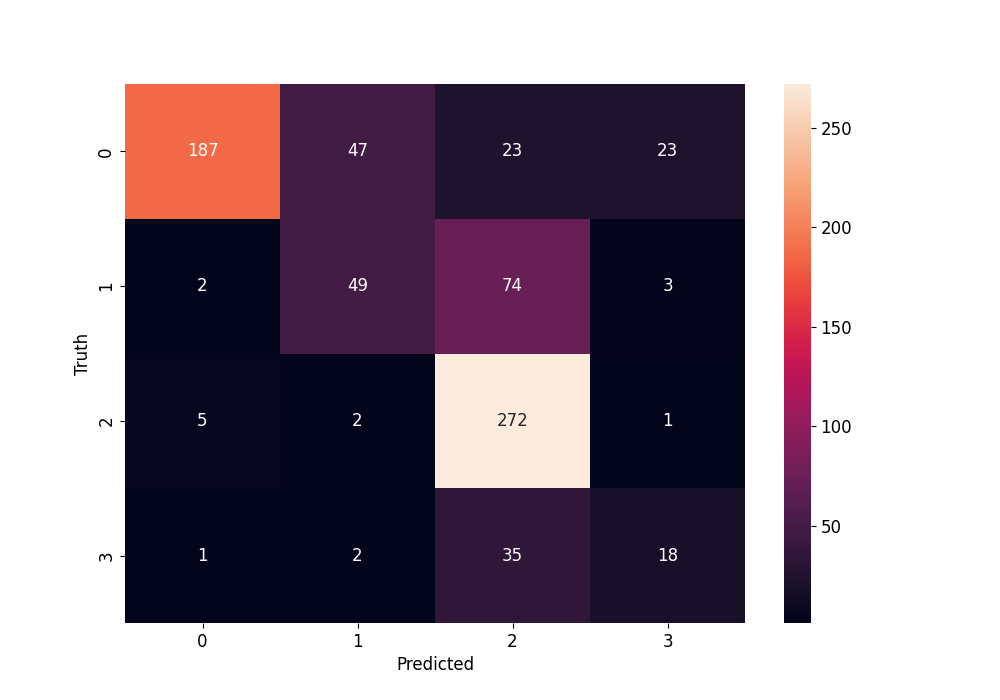
\includegraphics[scale=0.75]{figures/CM4.png}
	\caption{Matriz de confusión del modelo con 4 clases}
	\label{fig:img18}
\end{figure}

Al observar la figura 17, se resalta una disminución en la pérdida en validación, que anteriormente convergía aproximadamente en los valores de 1.0 y ahora se acerca a 0.5. En la gráfica de exactitud, por primera vez se logró superar el 80\% en validación. Además, el comportamiento de la exactitud se aprecia de manera visible en la matriz de confusión en la figura 18.\par

A continuación se muestran las gráficas descriptivas para el modelo de 3 clases:

\begin{figure}[H]
	\centering
	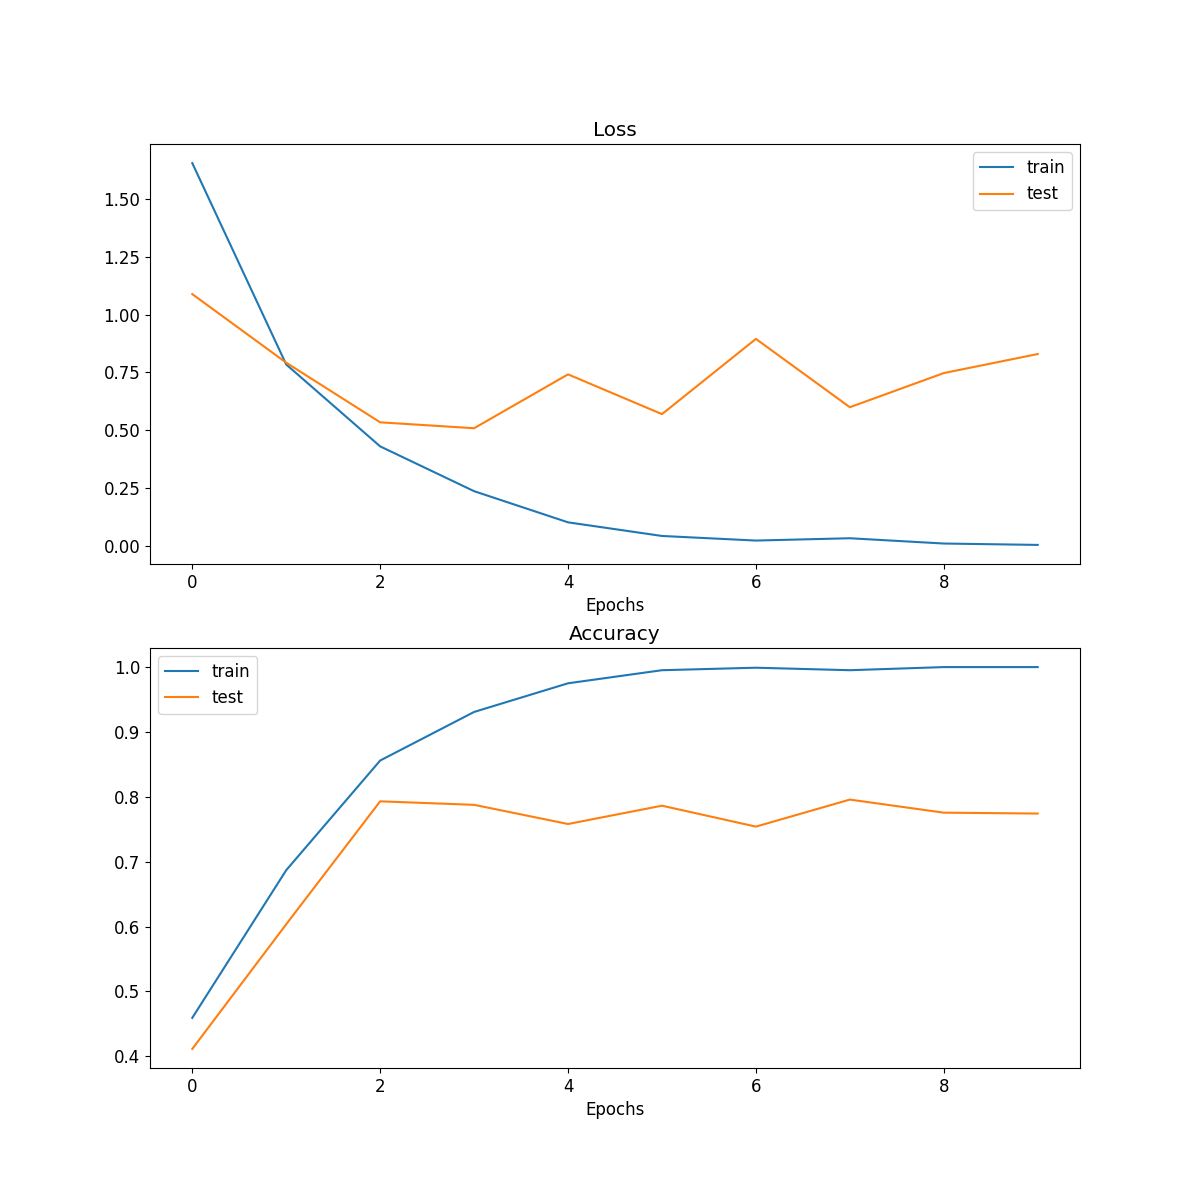
\includegraphics[scale=0.65]{figures/LA5.png}
	\caption{Pérdida y exactitud del modelo con 4 clases}
	\label{fig:img19}
\end{figure}

\begin{figure}[H]
	\centering
	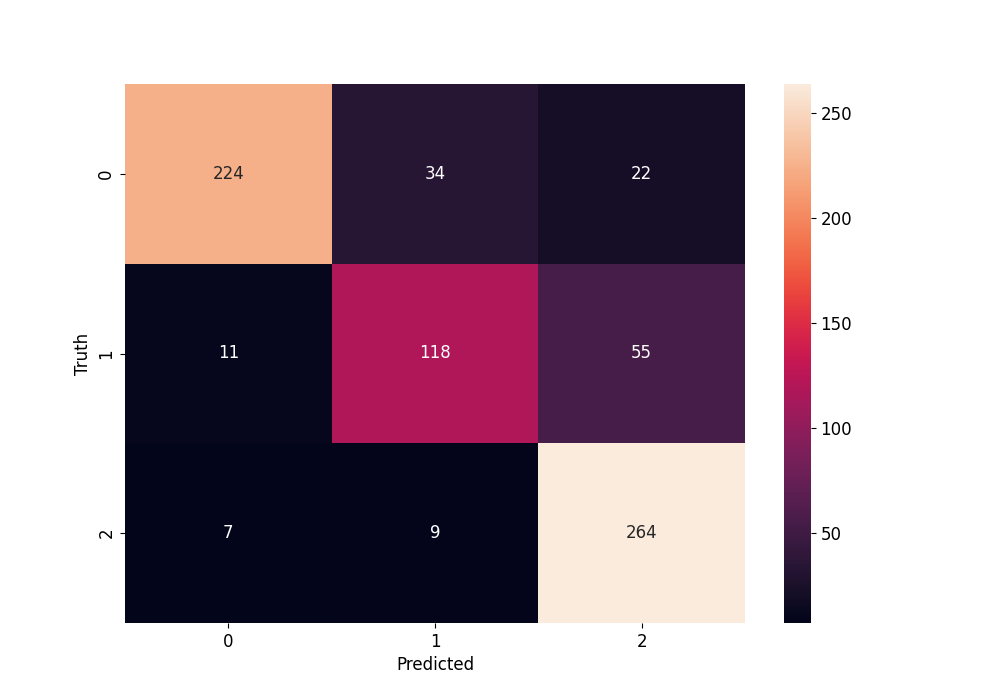
\includegraphics[scale=0.75]{figures/CM5.png}
	\caption{Matriz de confusión del modelo con 4 clases}
	\label{fig:img20}
\end{figure}

En la figura 19 se puede observar que la pérdida fluctúa entre los valores 0.5 y 0.1, lo cual es muy similar al modelo de 4 etiquetas. En la gráficas de exactitud, se observa que los datos predecidos nuevamente generan una exactitud levemente superior al 80\%. Por otro lado, en la matriz de confusión en la figura 20, se observa que las magnitudes de los aciertos son similares entre sí respecto de las clases. En general el modelo de 3 clases tiene una buena base teórica para funcionar con el usuario Gerardo Fuentes, sin embargo utilizar 4 clases resulta más útil a nivel de comandos. \par


\subsubsection{Tercer grupo de modelos de aprendizaje}

En este grupo de modelos, se utiliza la misma configuración para la red neuronal que en los modelos anteriores. Sin embargo, en este caso se incrementó la cantidad de datos para entrenamiento, se utilizan 4 clases en todos los modelos, el octavo modelo utiliza filtros y el noveno fue cargado con imágenes de sujetos de prueba que utilizan marcadores faciales, los cuales se explican en la sección de bases de datos y fotografías personales. A continuación se muestran los resultados de los modelos:

\begin{figure}[H]
	\centering
	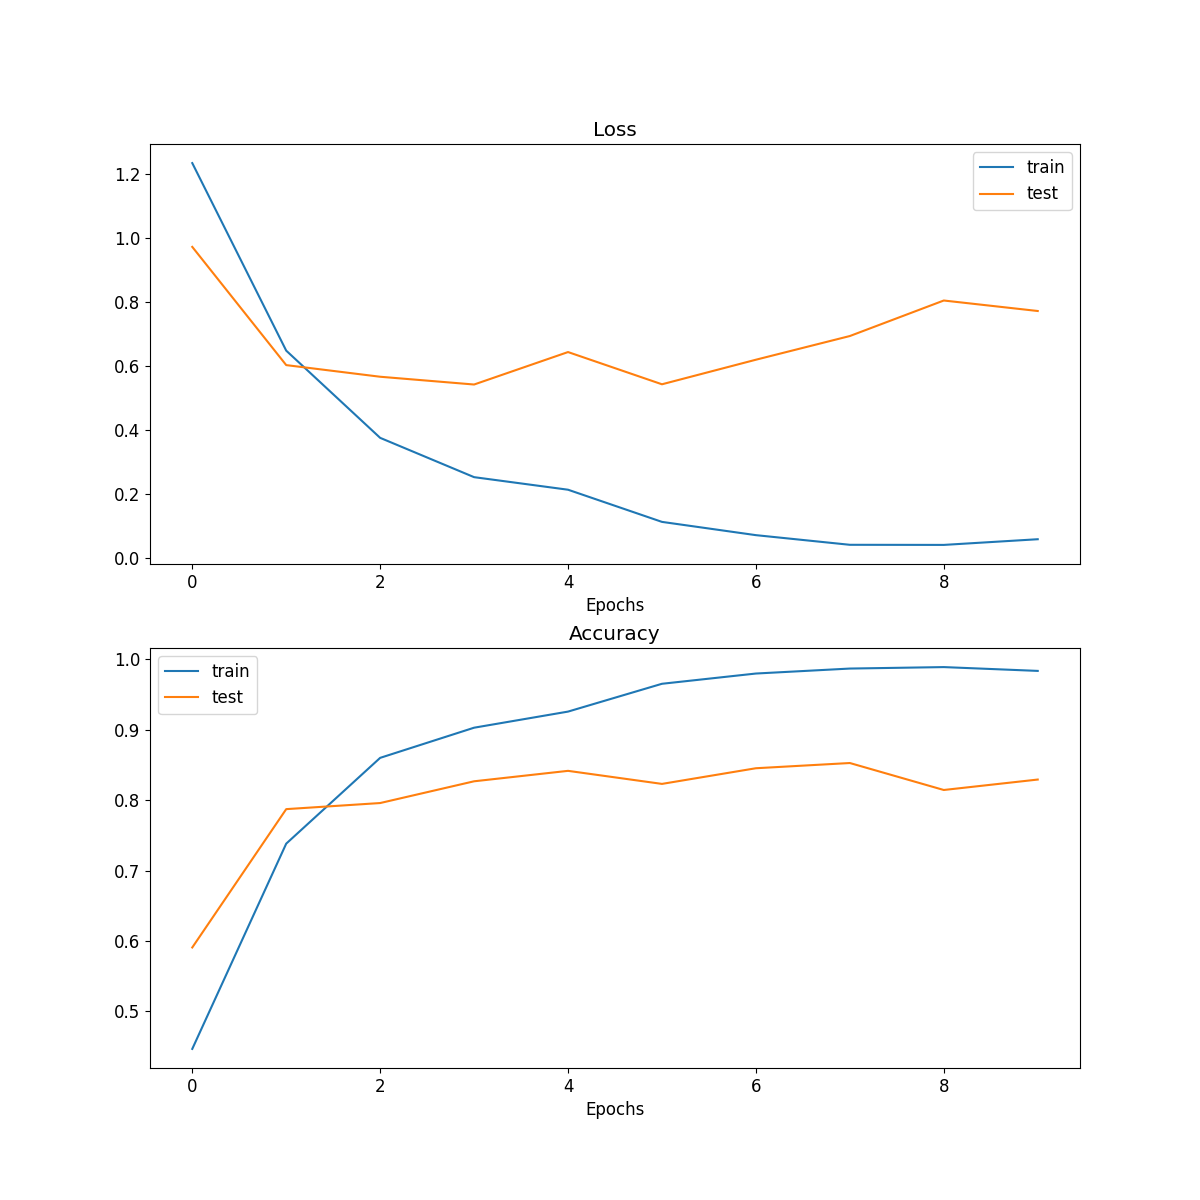
\includegraphics[scale=0.65]{figures/LA6.png}
	\caption{Pérdida y exactitud del modelo con 4 clases y aumento de imágenes de entrenamiento}
	\label{fig:img21}
\end{figure}

\begin{figure}[H]
	\centering
	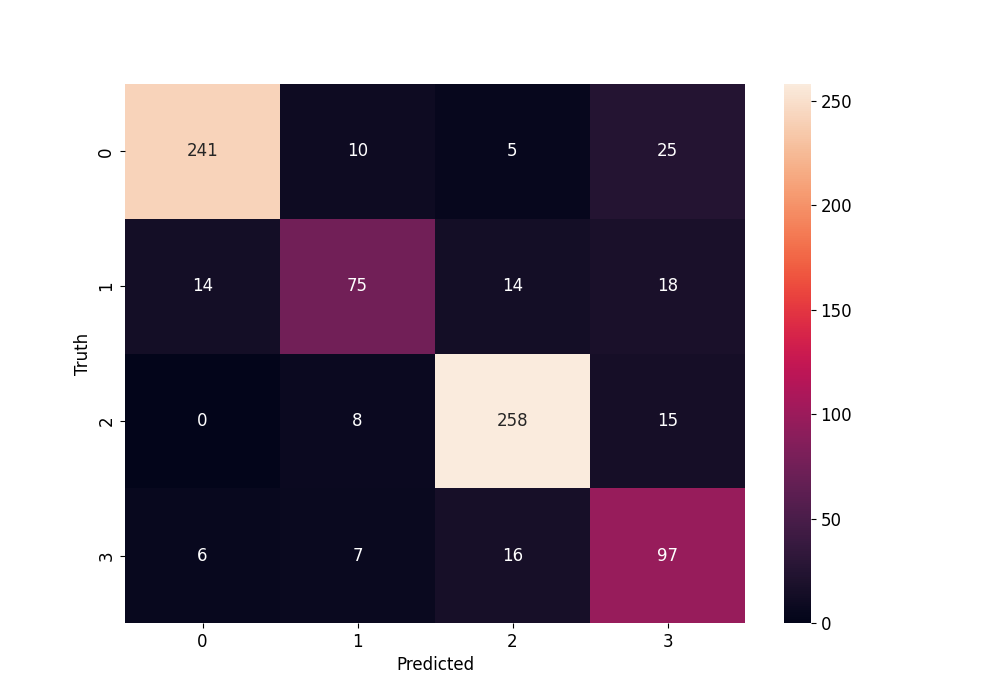
\includegraphics[scale=0.75]{figures/CM6.png}
	\caption{Matriz de confusión del modelo con 4 clases y aumento de imágenes de entrenamiento}
	\label{fig:img22}
\end{figure}

En la figura 21 se puede observar que los valores de pérdida por primera vez lograron valores menores a 1.0, y la exactitud logra superar el 80\% de aciertos. Además la matriz de confusión de la figura 22 muestra una diagonal de aciertos mucho más clara. 

\begin{figure}[H]
	\centering
	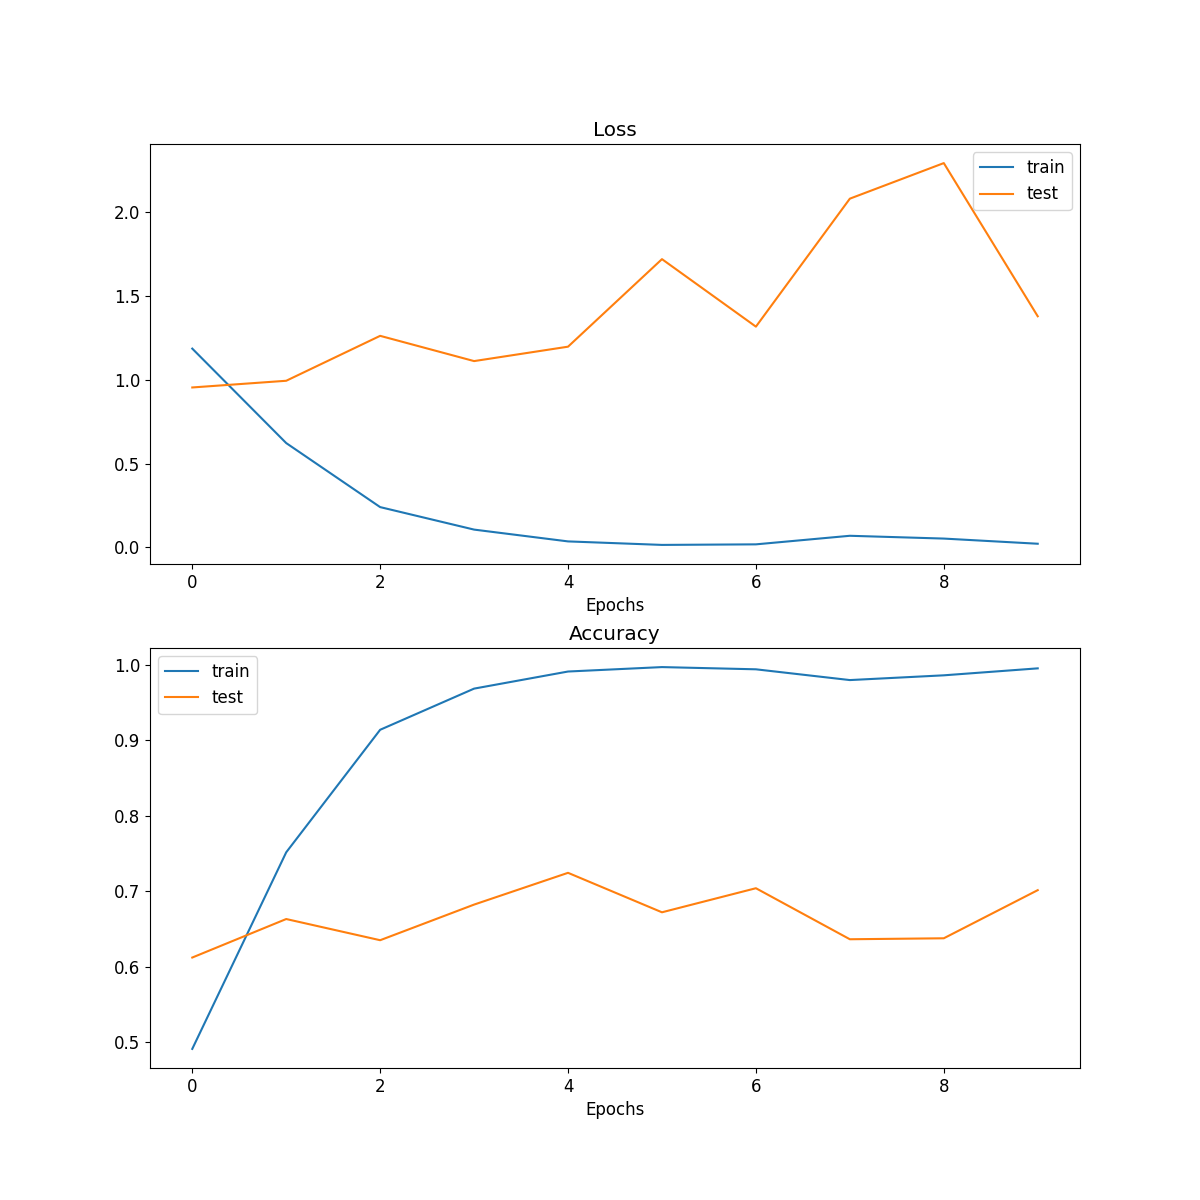
\includegraphics[scale=0.65]{figures/LA7.png}
	\caption{Pérdida y exactitud del modelo con 4 clases con filtro de bordes}
	\label{fig:img23}
\end{figure}

\begin{figure}[H]
	\centering
	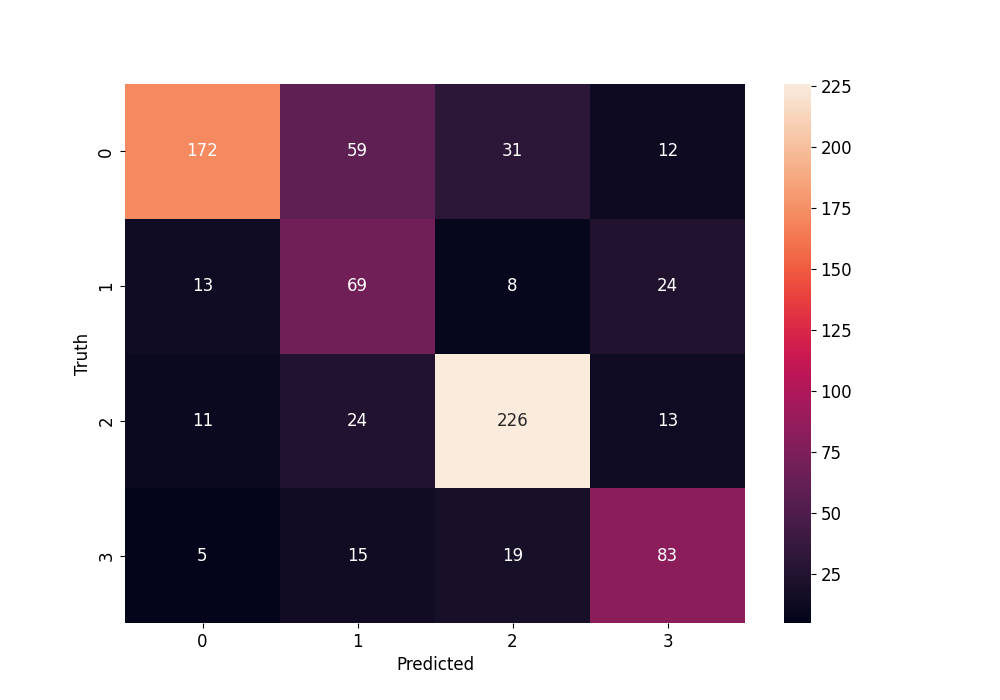
\includegraphics[scale=0.75]{figures/CM7.png}
	\caption{Matriz de confusión del modelo con 4 clases con filtro de bordes}
	\label{fig:img24}
\end{figure}

En este caso se puede observar el octavo modelo, el cual incluye un filtro de bordes para las fotografías. En la figura 23, se muestra un claro paso atrás en la disminución de valores de pérdida, superando nuevamente el valor de 1.0, mientras que para la exactitud de aciertos, el porcentaje queda aún menor a 70\%. Este comportamiento erróneo es visible en la matriz de confusión de la figura 24.

\begin{figure}[H]
	\centering
	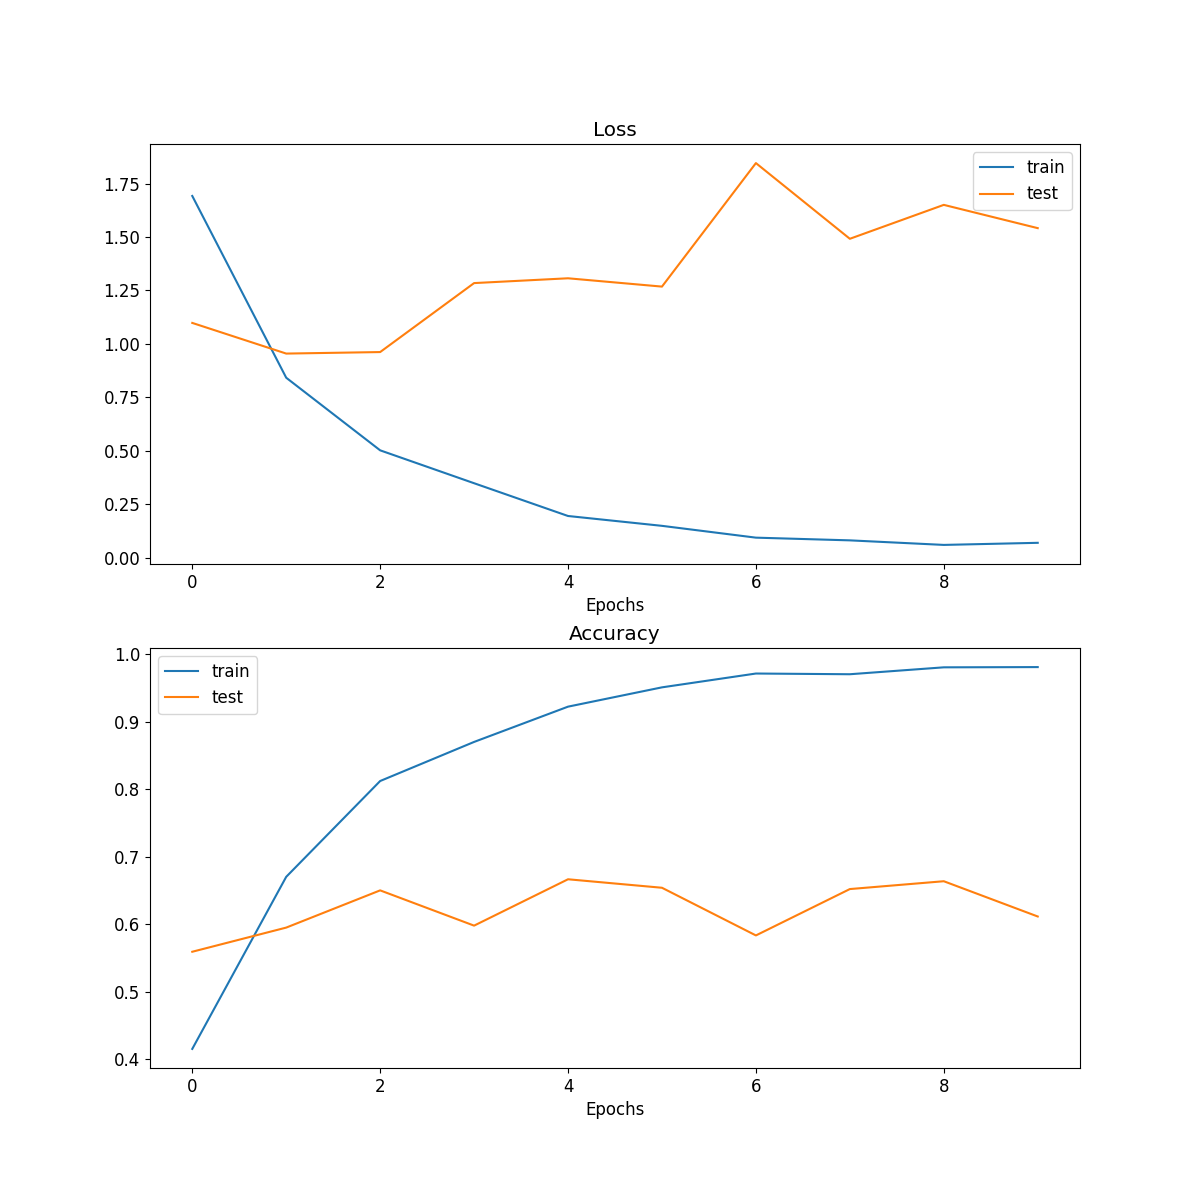
\includegraphics[scale=0.65]{figures/LA8.png}
	\caption{Pérdida y exactitud del modelo con 4 clases y marcadores faciales}
	\label{fig:img25}
\end{figure}

\begin{figure}[H]
	\centering
	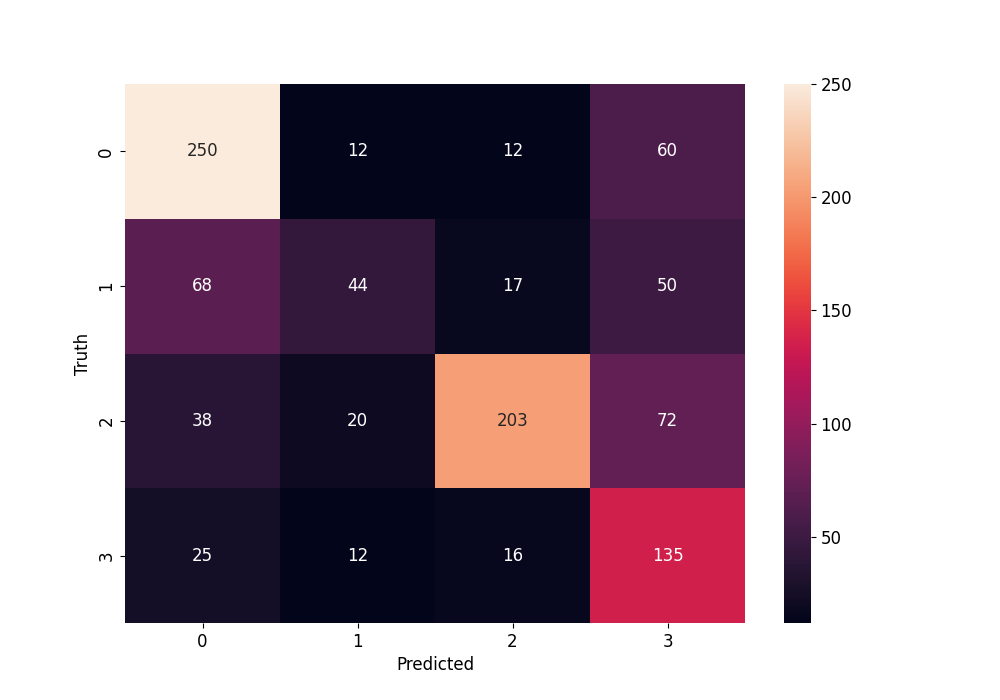
\includegraphics[scale=0.75]{figures/CM8.png}
	\caption{Matriz de confusión del modelo con 4 clases y marcadores faciales}
	\label{fig:img26}
\end{figure}

Para este noveno modelo, en la figura 25 el resultado de pérdida nuevamente supera el valor de 1.0, y la exactitud no supera el 70\%. Sin embargo, la matriz de confusión muestra un comportamiento más claro que el octavo modelo en cuanto a la diagonal de aciertos. Esto último tiene que ver con el incremento de imágenes obtenidas de los 10 sujetos de prueba. 
